\documentclass[10pt,a4paper]{article}
\usepackage[latin1]{inputenc}
\usepackage{amsmath}
\usepackage{amsfonts}
\usepackage{amssymb}
\usepackage{graphics}
\usepackage{hyperref}
\usepackage{fullpage}
\def\Version#1{\def\version{#1}}
\author{Gergely Imreh}
\Version{1.1}
\title{Optimal Zeeman-slower length, \version}
\begin{document}
\maketitle

Here I'll summarize the calculations for determining the optimal Zeeman-slower length in the case where the length of collimator tube is adjusted to always match the slower aspect ratio.

When the length of the slower is changed there are two effects to take into account: longer slower can capture a higher fraction of the thermal distribution, but a smaller but the matching collimator will have smaller flux.

For a large part of this calculation I used Mathematica, but checked everything numerically afterwards.

\section{Velocity capture}

The optimal slowing acceleration by the Doppler-cooling laser is
\begin{equation}
a_D = \frac{\hbar k \Gamma}{2 m}
\end{equation}
where $k$ is the cooling transition's wavenumber, $\Gamma$ is the transition linewidth and $m$ the atom's mass. The length of the slower for initial and final velocities $v_0$ and $v_f$ is
\begin{equation}
L = \frac{v_0^2 - v_f^2}{2 \eta a_D}
\end{equation}
and thus the maximum capture velocity as a function of slower length is expressed as
\begin{equation}
v_0 = \sqrt{2 \eta a_D L + v_f^2} = \sqrt{A L + B}
\end{equation}
where $A = 2 \eta a_D$ and $B = v_f^2$. The Maxwell-Boltzmann distribution of the atomic beam is
\begin{equation}
f \sim v^3 \exp\left(-\frac{v^2}{u^2}\right) = v^3 \exp(-C v^2)
\end{equation}
where $u = \sqrt{2 k_B T / m}$ and $C = 1/u^2$. After normalization the expression is
\begin{equation}
f = \frac{v^3}{2 C^2} \exp(-C v^2).
\end{equation}
For a given maximum velocity $v_0$ the capture fraction is
\begin{equation}
p(v_0) = \int_0^{v_0} f dv = 1 - \exp(-C v_0^2)(1 + C v_0^2).
\end{equation}
Here the slower length can be substituted to arrive to
\begin{equation}
p_v(L) = 1 - \exp(-C (A L + B))(1 + C (A L + B))
\label{eq:velocityfraction}
\end{equation}
and
\begin{equation}
\frac{\partial p_v}{\partial L} = A C^2 (A L + B)\exp(-C (A L + B)) 
\end{equation}

\section{Angular distribution}

I had to fix the expression for the angular distribution from the previous document that had some problems that didn't show up in the simulations. The new expression for the capture fraction at an angle $\theta$:
\begin{equation}
f(\theta) =  \left(2 r^2 \arccos\left(\frac {l \tan(\theta)}{2 r} \right) - \frac{l \tan(\theta)}{2}\sqrt{4 r^2 - L^2 \tan^2(\theta)}\right) / r^2 \pi
\end{equation}
where $r$ and $l$ are the collimator pinhole size and length, respectively. Substitute the parameter $t = \tan(\theta)$ and the integration limit is $t \in [0, 2 r / l]$. We would normally have to take into account the distribution $\cos(\theta)$ distribution of the atomic velocities out of the pinhole, but for small $\theta$ it is very close to 1, so here I ignore it. For slower lengths above 2cm this seems to be a good approximation, since all practical slowers are much longer than that.

The total capture fraction (in the small $\theta$ approximation) is
\begin{equation}
p_a(l) = \int_0^{2r/l} f(t) dt = \frac{8 r}{3 \pi l}.
\end{equation}
Since the collimator length is always optimized for the Zeeman slower, that is the maximum angle matches the aspect ratio defined by the half spot size ($r_{\rm spot}/2$) and slower length $L$:
\begin{equation}
l = \frac{2 r L}{r_{\rm spot} / 2}.
\end{equation}
Thus the capture fraction becomes
\begin{equation}
p_a(L) = \frac{2 r_{\rm spot}}{3 \pi L}.
\label{eq:anglefraction}
\end{equation}
and
\begin{equation}
\frac{\partial p_a}{\partial L} = -\frac{2 r_{\rm spot}}{3 \pi L^2}
\end{equation}
If there's a buffer length before and/or after the slower with total length $D$:
\begin{eqnarray}
p_a(L) &=& \frac{2 r_{\rm spot}}{3 \pi (L+D)} \\
\frac{\partial p_a}{\partial L} &=& -\frac{2 r_{\rm spot}}{3 \pi (L+D)^2}
\end{eqnarray}


\section{Combination}
The total capture fraction from Eq. \ref{eq:velocityfraction} and \ref{eq:anglefraction} is
\begin{equation}
p = p_v \times p_a = -\frac{2 r_{\rm spot} (1 - \exp(-C (A L + B))(1 + C (A L + B)))}{3 \pi L}
\label{eq:flux}
\end{equation}
and
\begin{eqnarray}
\frac{\partial p}{\partial L} &=& \frac{\partial p_v}{\partial L} p_a + p_v \frac{\partial p_a}{\partial L} \\
  &=&-\frac{2 \exp(-C (A L + B))  r_{\rm spot}}{3 L^2 \pi }\left(\exp(C (A L+B))-A C L - (A C L)^2-B C (1+A C L) - 1\right)
\label{eq:dflux}
\end{eqnarray}
and $p$ has extreme value when
\begin{equation}
X(L) = \exp(C (A L+B))-A C L - (A C L)^2-B C (1+A C L) - 1 == 0
\end{equation}
Mathematica can not find an algebraic solution to this, but numerically it is solved easily. Since this expression is continuous and
\begin{eqnarray}
X(0) =& -BC &< 0 \\
X(L\gg1) =& \exp(C (AL+B)) &> 0
\end{eqnarray}
there has to be a sign change between $(0 < L < \infty)$ thus there's always a zero crossing, meaning there's always a maximum value of the flux at finite $L$.


In the case of buffer space case the expression goes as
\begin{eqnarray}
\frac{\partial p}{\partial L} &=& \frac{\partial p_v}{\partial L} p_a + p_v \frac{\partial p_a}{\partial L} \\
  &=&-\frac{2 \exp(-C (A L + B))  r_{\rm spot}}{3 (L+D)^2 \pi } \times \nonumber \\
  & &\left(\exp(C (A L+B))-A C L - A^2 C^2 D L- (A C L)^2-B C (1+A C (L+D)) - 1\right)
\end{eqnarray}
and $p$ has extreme value when
\begin{equation}
X(L) = \exp(C (A L+B))-A C L - A^2 C^2 D L - (A C L)^2 - B C (1+A C L) - 1 == 0
\end{equation}


\begin{figure}[ht]
\centering
\resizebox{0.8\columnwidth}{!}{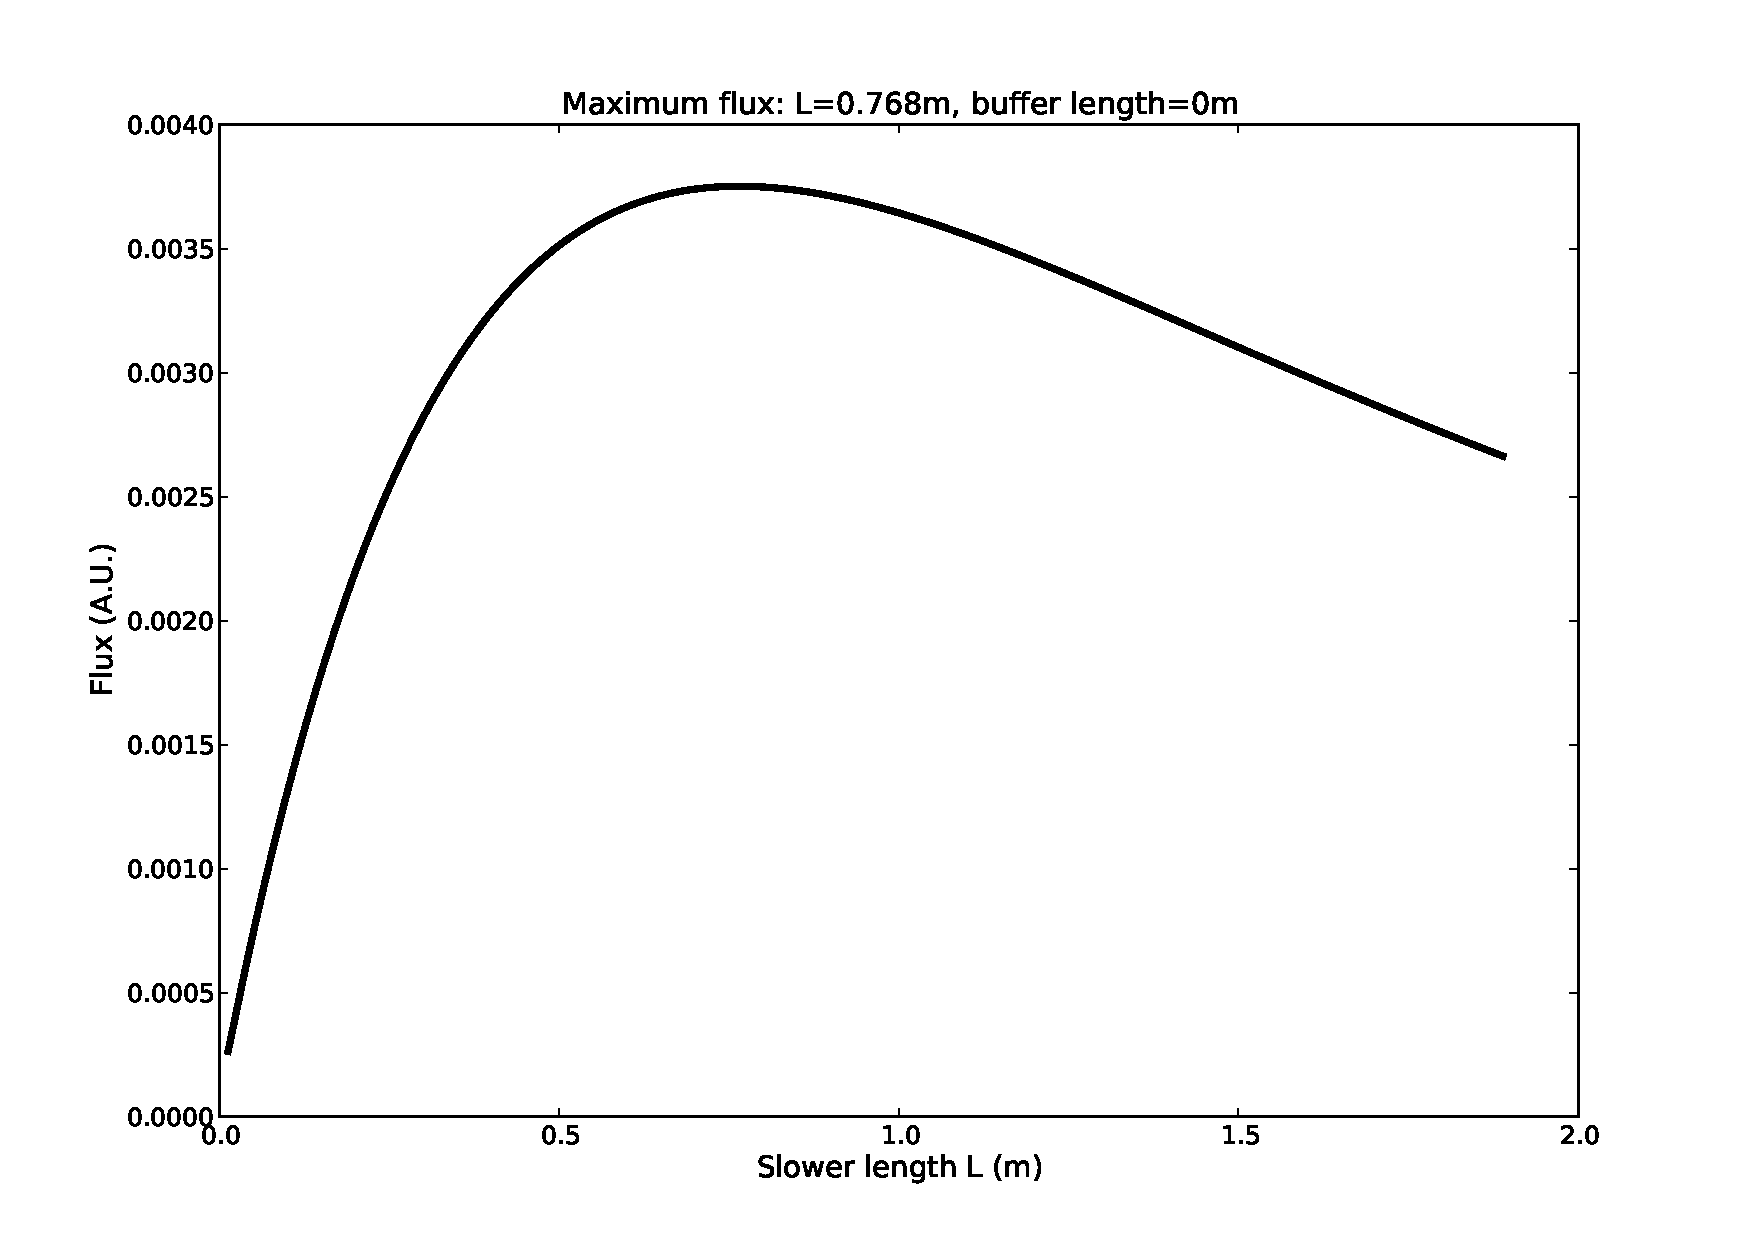
\includegraphics{newflux.pdf}}
\caption{Flux as a function of slower length, for the case of no buffer space, see Eq. \ref{eq:flux}.}
\label{fig:flux}
\end{figure}


\begin{figure}[ht]
\centering
\resizebox{0.8\columnwidth}{!}{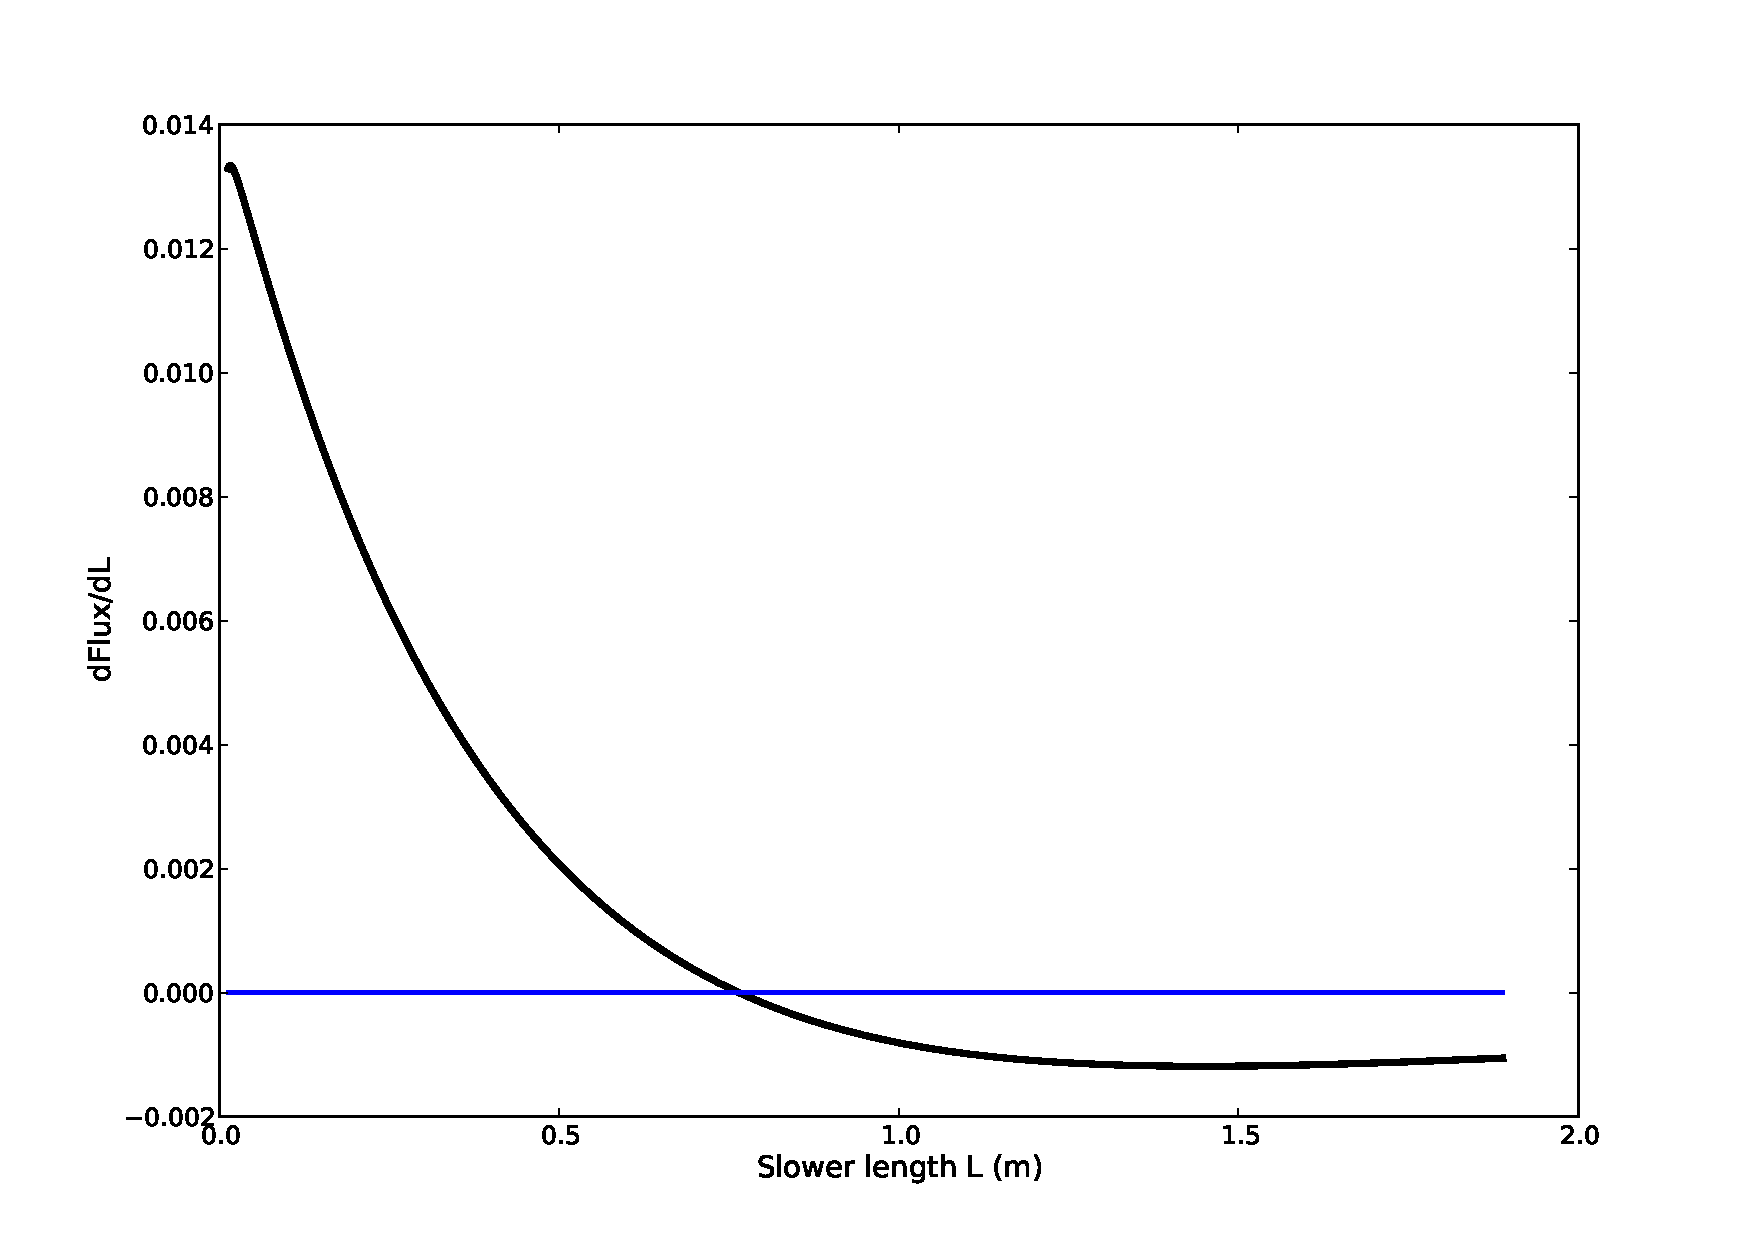
\includegraphics{newfluxd.pdf}}
\caption{The first derivate of the flux by the slower length, see Eq. \ref{eq:dflux}.}
\label{fig:dflux}
\end{figure}



\end{document}